\section{Spark Internals}

\subsection{Example walk-through}
\begin{frame}
\begin{figure}
\centering
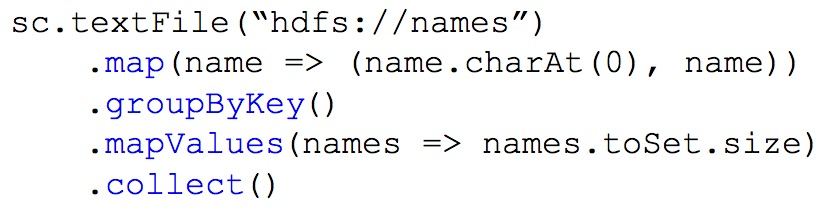
\includegraphics[width=0.8\linewidth]{figures/example2.jpg}
\caption{Find number of distinct names per ``first letter''. This example is
reproduced from [3].}
\end{figure}
\end{frame}

\begin{frame}
\begin{figure}
\centering
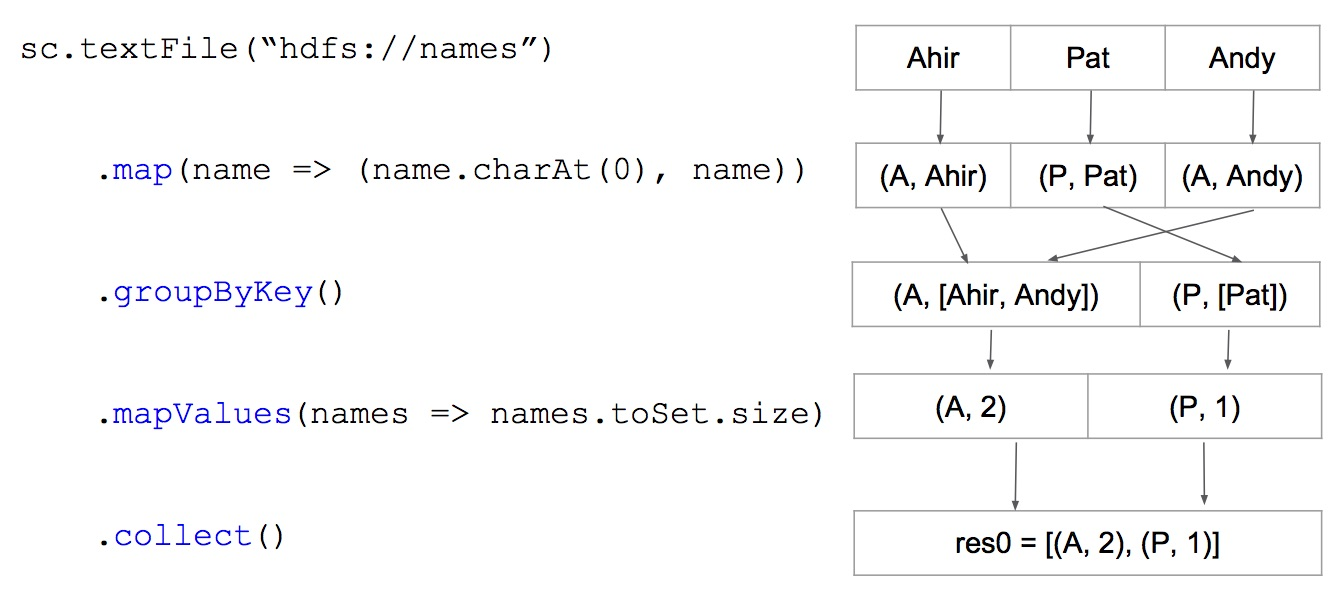
\includegraphics[width=0.9\linewidth]{figures/example2-wall-through.jpg}
\end{figure}
\end{frame}

\subsection{Lineage of RDDs}
\begin{frame}
\begin{figure}
\centering
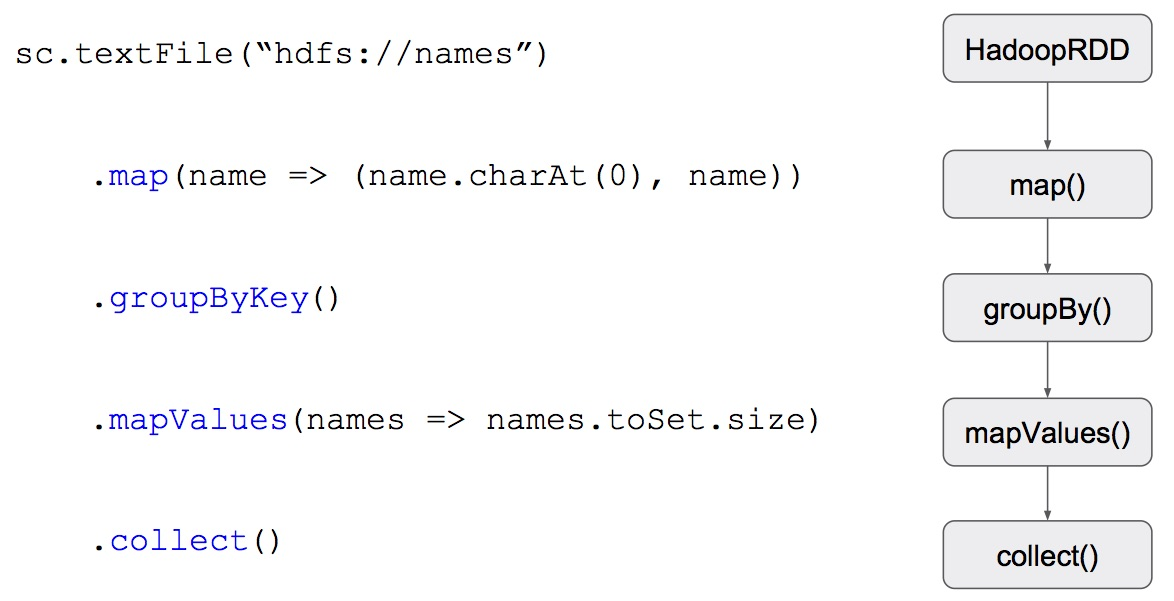
\includegraphics[width=0.9\linewidth]{figures/example2-rdd-dag.jpg}
\end{figure}
\end{frame}

\subsection{Staging}
\begin{frame}
\begin{figure}
\centering
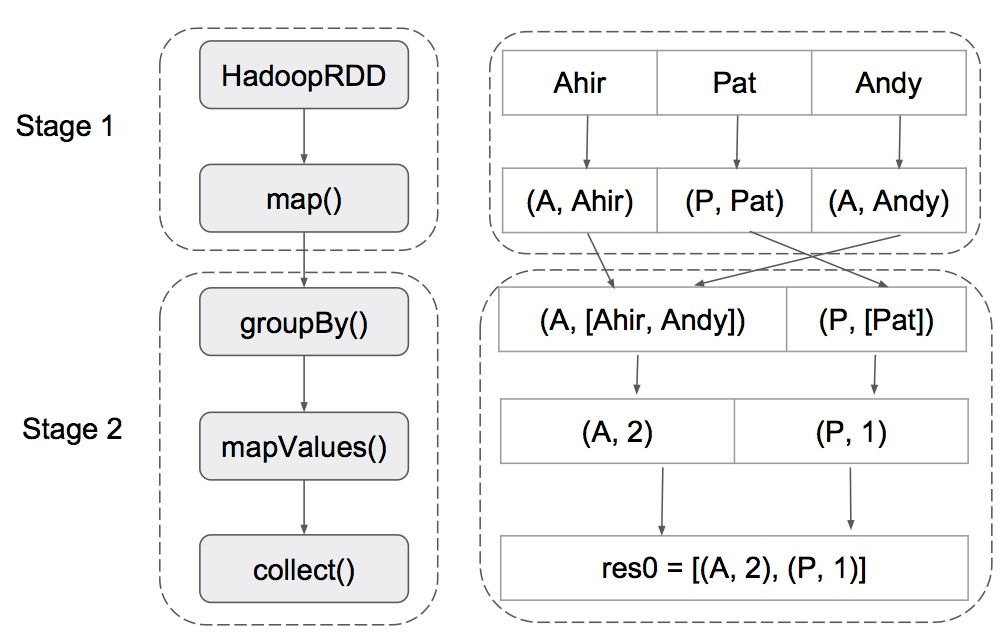
\includegraphics[width=0.6\linewidth]{figures/example2-staging.jpg}
\end{figure}
\end{frame}

\subsection{Execution Model}
\begin{frame}
\begin{figure}
\centering
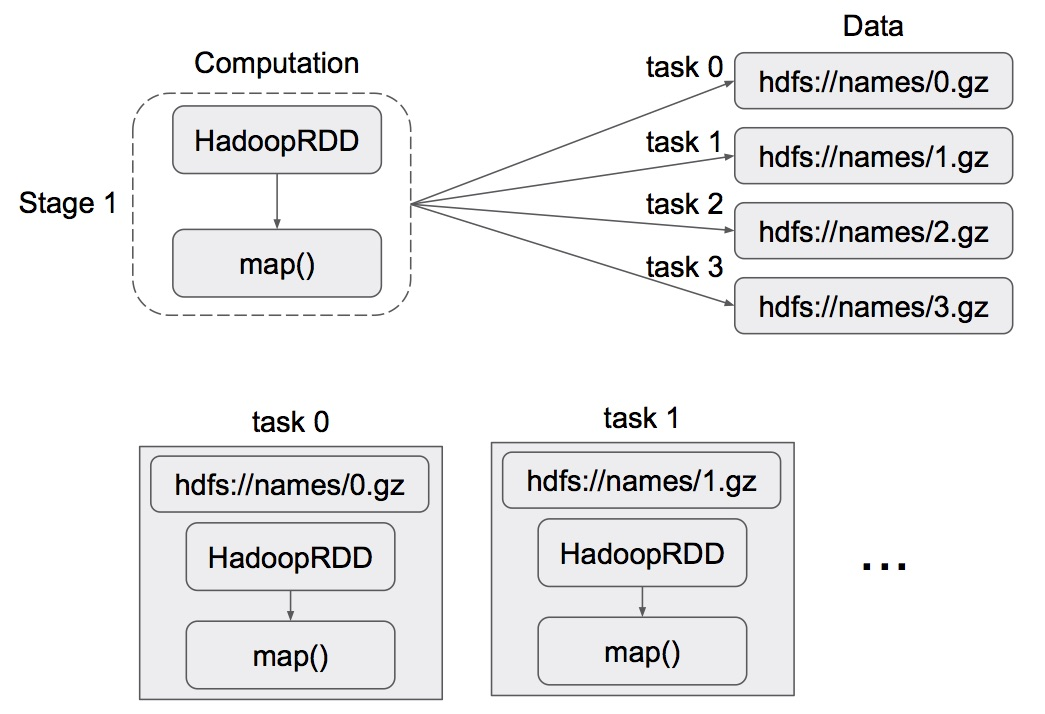
\includegraphics[width=0.8\linewidth]{figures/example2-tasking.jpg}
\end{figure}
\end{frame}

\subsection{Scheduling}
\begin{frame}
\begin{figure}
\centering
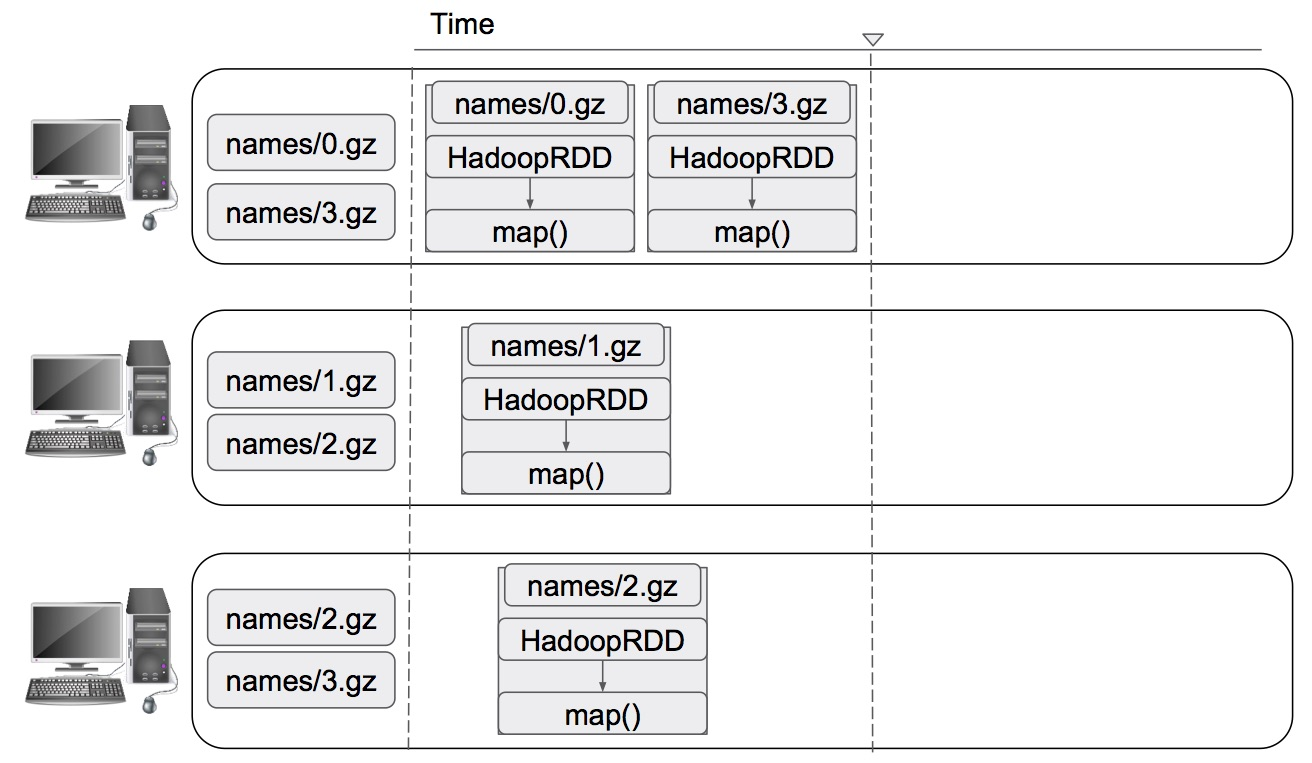
\includegraphics[width=0.9\linewidth]{figures/example2-scheduling.jpg}
\end{figure}
\end{frame}

\subsection{Shuffling}
\begin{frame}
\begin{figure}
\centering
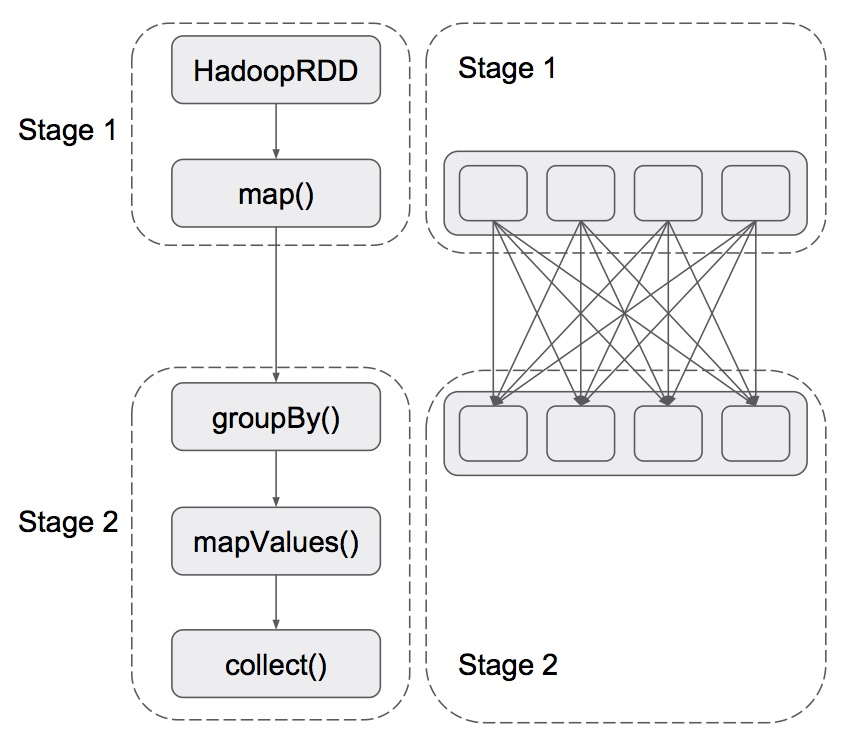
\includegraphics[width=0.6\linewidth]{figures/example2-shuffling.jpg}
\end{figure}
\end{frame}


\begin{frame}
\begin{figure}
\centering
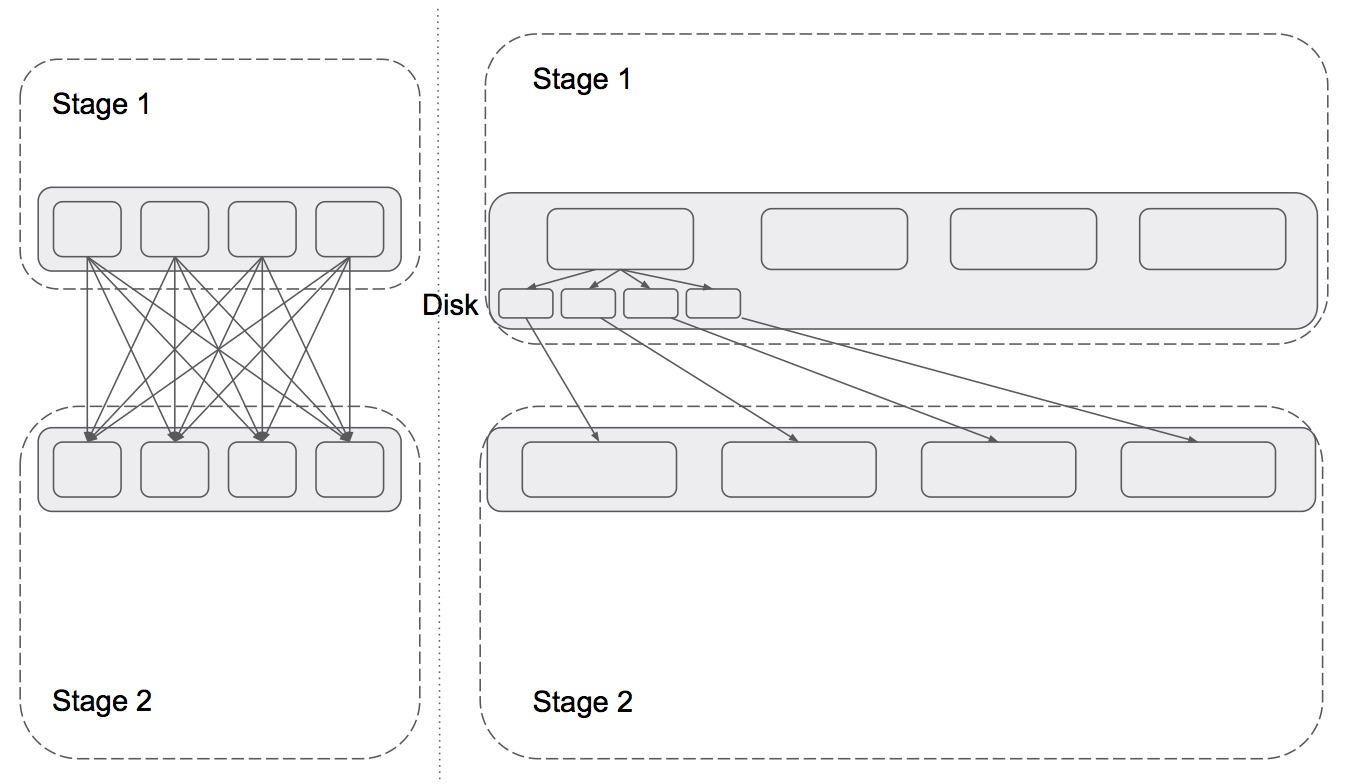
\includegraphics[width=0.9\linewidth]{figures/example2-shuffling-details.jpg}
\end{figure}
\end{frame}